\documentclass[11pt, oneside]{article}
\usepackage{geometry}
\geometry{letterpaper, margin=0.8in,top=0.75in}
\usepackage[utf8]{inputenc}
\usepackage[english]{babel}

\usepackage{amsmath}
\usepackage{amssymb}
\usepackage{amsthm}
\usepackage[ruled,vlined]{algorithm2e}
\usepackage{graphicx}
\usepackage{siunitx}
\usepackage{booktabs}
\usepackage{array}
\usepackage{subcaption}
\usepackage{xcolor}
% \usepackage{natbib}

\definecolor{ForestGreen}{cmyk}{0.83,0.21,1,0.08}
\definecolor{ONTech-dark-blue}{cmyk}{1,0.58,0.09,0.46}
\definecolor{ONTech-light-blue}{cmyk}{1,0.31,0,0}
\definecolor{ONTech-orange}{cmyk}{0,0.70,1,0}
\definecolor{ONTech-warm-grey}{cmyk}{0.9,0.11,0.13,0.20}
\definecolor{ONTech-cool-grey}{cmyk}{0.20,0.14,0.12,0.40}
\definecolor{ONTech-dark-grey}{cmyk}{0.45,0.25,0.16,0.59}
\definecolor{ONTech-navy}{cmyk}{1,0.75,0.50,0.50}

\title{ Reduced Basis Method for Parametrized Partial Differential Equations\\
        \normalsize MCSC 6020G - Numerical Analysis}
\author{Parikshit Bajpai}
\date{}

\newtheorem*{remark}{}
\newtheorem*{order}{Complexity}
\renewcommand\qedsymbol{$\blacksquare$}

\begin{document}
\maketitle

\section{Introduction}
Parametrised models implicitly connect the input parameters characterising a problem, such as physical properties, boundary conditions, etc., to the outputs of interest, such as maximum system temperature, channel flow rate, etc. Accurate high-fidelity tools are of broad interest to allow the solution of such problems, but in many situtations, such as many-query design evaluations, the solution is sought for a large number of different parameter values. The high-fidelity models are often computationally expensive and time consuming for such simulations a different approach is required to allow the evaluation of the desired output at minimal cost, yet without sacrificing the predictive accuracy of the complex model.

A class of methods, known as Reduced Basis (RB) methods, accomplish this by building on the high-fidelity model to effectively represent the parametrised solutions in terms of suitable problem dependent basis functions.

This project demonstrates the use of RB method in finding linear functional output of a affine linear elliptic coercive partial differential equation (heat conduction) using a thermal block toy problem and presents a very simple application to fluid flow in a backward-facing step channel.

\section{Parametrised Differential Equation}
The abstract formulation of the problem of interest in parametric weak formulation can be written as follows \cite{quarteroni2017}:

$\text{Given parameter } \mu \in \mathbb{P} \text{, find }u(\mu) \in \mathbb{V} \text{ such that }$
\begin{equation}\label{eq:1}
  a(u(\mu), v; \mu) = f(v;\mu)  \mspace{5mu} \forall v \in \mathbb{V}
\end{equation}
$\text{and evaluate}$
\begin{equation}\label{eq:2}
  s(\mu) = l(u(\mu);\mu)
\end{equation}
where, $f:\mathbb{V} \times \mathbb{P} \rightarrow \mathbb{R}$ and $l:\mathbb{V} \times \mathbb{P} \rightarrow \mathbb{R}$ are parameterized linear forms and $a:\mathbb{V} \times \mathbb{V} \times \mathbb{P} \rightarrow \mathbb{R}$ is a bilinear form.

The discrete approximation to parametric weak formulation \ref{eq:1} is sought in the discrete approximation space $\mathbb{V}_{\delta} \subset \mathbb{V}$ which can be constructed, for example, as a standard finite element method using piece-wise linear functions. For the development of the most simple reduced basis model as used in this project, the discrete space is assumed to be conforming \cite{HesthavenRozzaStamm2015}. Denoting the dimension of the discrete space $\mathbb{V}_{\delta}$ by $N_{\delta} = \text{dim}{\mathbb{V}}$ and equiping $\mathbb{V}_{\delta}$ with a basis $\{\psi_i\}_{i=1}^{N_\delta}$, the discrete problem can then be formulated as:

$\text{For each } \mu \in \mathbb{P} \text{, find } u_{\delta}(\mu) \in \mathbb{V}_{\delta} \text{ such that }$
\begin{equation}\label{eq:3}
  a(u_{\delta}(\mu), v_{\delta}; \mu) = f(v_{\delta};\mu)  \mspace{5mu} \forall v_{\delta} \in \mathbb{V_{\delta}}
\end{equation}
$\text{and evaluate}$
\begin{equation}\label{eq:4}
  s_{\delta}(\mu) = l(u_{\delta}(\mu);\mu)
\end{equation}

The discrete problem is often denoted as the \textit{truth problem} and its solution, called the \textit{truth approximation}, can be achieved with as high accuracy as desired. However, the computation of the truth solution is very expensive since the space $\mathbb{V}_{\delta}$ can have extremely large degrees of freedom. This model is also referred to as the \textit{high fidelity model}.

\section{Reduced Basis Method}
With target applications characterised by computationally intensive parametrised problems that require repeated evaluation, reduced basis methods provide a low-cost alternative. The final goal of RB methods is to approximate any member of this solution manifold with a low number of, say N , basis functions. This set of basis functions is denoted as the reduced basis \cite{HesthavenRozzaStamm2015}.

The essential ingredients of RB methodology are: a Galerkin projection onto a low-dimensional space of properly selected basis functions, an affine parametric dependence enabling to perform a Offline-Online splitting in the computational procedure, and a rigorous \textit{a posteriori} error estimation used for both the basis selection and the certification of the solution. The combination of these three factors yields substantial computational savings which are at the basis of an efficient model order reduction, ideally suited for real-time simulation and many-query contexts (for example, optimization, control or parameter identification) \cite{quarteroni2011}.

\subsection{Reduced basis approximation}
The end goal of RB method is to represent the truth solution based on a $N$ dimensional subspace $\mathbb{V}_{rb}$ of $\mathbb{V}_{\delta}$, where $N \ll N_{\delta}$ and the reduced basis space is given by
    \begin{equation}
      \mathbb{V}_{rb} = \text{span}\{\xi_1,\dots,\xi_N\} \subset \mathbb{V}_{\delta}
    \end{equation}
    where, $\{\xi_n\}_{n=1}^{N} \subset \mathbb{V}_{\delta}$ denote the reduced basis functions.The reduced basis problem is given as follows.

For any given $\mu \in \mathbb{P}$, find $u_{rb}(\mu) \in \mathbb{V}_{rb}$ such that
  \begin{equation}
        {a}(u_{rb}(\mu), v_{rb}; \mu) ={f}(v_{rb};\mu) \mspace{20mu} \forall v_{rb} \in \mathbb{V}_{rb}
  \end{equation}
and evaluate
  \begin{equation}
    \mathrm{s}_{rb}(\mu) = \mathrm{f}(u_{rb}(\mu);\mu)
  \end{equation}

Since the basis functions of $\mathbb{V}_{rb}$ are given by $\xi_1,\dots,\xi_N$, we can represent $u_{rb}(\mu) = \sum_{n=1}^{N}(u_{rb}^{\mu})_n \xi_n$ where $\{(u_{rb}^{\mu})_n\}_{n=1}^{N}$ denote the coefficients of the reduced basis approximation. The reduced basis method is explained at the level of linear through the followiing discussion.

Let $\{\xi_n\}_{n=1}^{N}$ denote the reduced basis and define matrix $\mathbf{B} \in \mathbb{R}^{N_{\delta} \times N}$ such that
    \begin{equation}
      \xi_n = \sum_{i=1}^{N_{\delta}} \mathbf{B}_{in} \psi_i
    \end{equation}
i.e., the n-th column of $\mathbf{B}$ denotes the coefficients when the n-th basis function $\xi_n$ is expressed in terms of the basis functions $\{\psi_i\}_{i=1}^{N_{\delta}}$. Then, the reduced basis solution matrix $\mathbf{A}_{rb}^{\mu} \in \mathbb{R}^{N \times N}$ and the right hand side $f_{rb}^{\mu} \in \mathbb{R}^{N}$ are defined by
    \begin{align}
      (\mathbf{A}_{rb}^{\mu})_{mn} = a(\xi_n, \xi_m; \mu) \\
      (f_{rb}^{\mu})_m = f(\xi_m;\mu) \mspace{25mu}  1\leq n,m \leq N
    \end{align}
where $ 1\leq n,m \leq N$ and the system of equations can be computed by
    \begin{align}
      \mathbf{A}_{rb}^{\mu} = \mathbf{B}^T \mathbf{A}_{\delta}^{\mu}\mathbf{B}\\
      f_{rb}^{\mu} = \mathbf{B}^T f_{\delta}^{\mu}
    \end{align}

The reduced basis approximation $u_{rb}^{\mu} = \sum_{n=1}^{N}(u_{rb}^{\mu})_n \xi_n$ is obtained by solving the linear system
    \begin{equation}
      \mathbf{A}_{rb}^{\mu}u_{rb}^{\mu} = f_{rb}^{\mu}
    \end{equation}
and the output of interest are evaluated as $s_{rb}(\mu) = (u_{rb}^{\mu})^T f_{rb}^{\mu}$

Some of the issues relating to the use of RB methods are the following:
\begin{itemize}
  \item How do we generate accurate reduced basis spaces during the offline phase.
  \item how do we recover the reduced basis solution efficiently suring the offline stage.
  \item What are the error estimates for the reduced basis solution.
\end{itemize}

A number of methods have been proposed to generate accurate reduced basis spaces. These include Proper Orthogonal Decomposition (POD), Greedy Algorithm, etc. Regarding recovering reduced basis solutions efficiently, the affine decomposition plays a key role in ensuring that the parameter can be separated from the bilinear and linear forms. The Empirical Interpolation Method is often used to perform such a decomposition in cases when the decomposition is not explicit. Finally, the maximum error bound depends on the coercivity and comntinuity constants of the bilinear-form, both of which are problem dependent. Since a number of references available in literature provide a detailed description of these methods and bounds, a discusssion of these has been omitted for brevity. Interested readers can refer to Quarteroni \textit{et al.} \cite{quarteroni2017,quarteroni2011}, Hesthaven \textit{et al.} \cite{HesthavenRozzaStamm2015}, etc.

\section{Heat Conduction in Thermal Block}
For the demonstration problem, we consider steady heat conduction in a two-dimensional domain $ \Omega = (-1,1) \times (-1,1)$ with outward pointing unit normal $\mathbf{n}$ on $\partial \Omega$. The boundary $\partial \Omega$ is split into three parts: the bottom $\Gamma_{base} = (-1,1) \times {-1}$ , the top $\Gamma_{top} = (-1,1) \times {1}$ and the sides $\Gamma_{side} = {\pm 1} \times (-1,1)$. The domain is divided into two sub-domains  $\Omega_0$ and $\Omega_1$, such that $\Omega_0$ is a disk centered at the origin of radius $r_0=0.5$, and $\Omega_1=\Omega/\ \overline{\Omega}_0$.The conductivity $\kappa$ is assumed to be constant on $\Omega_0$ and $\Omega_1$, i.e., $\kappa|_{\Omega_0}=\kappa_0 \text{ and } \kappa|_{\Omega_1}=1$. This setup has been shown in fig.~\ref{fig:1}
    \begin{figure}
        \centering
        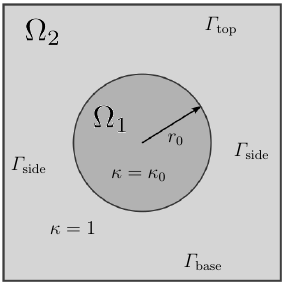
\includegraphics[width=0.5\textwidth]{figures/thermal_block.png}
        \caption{Geometrical set-up of the heat conductivity problem.}
        \label{fig:1}
    \end{figure}

For this problem, we consider $P=2$ parameters, the first one related to the conductivity in $\Omega_0$, i.e. $\mu_0\equiv k_0$, and the second parameter $\mu_1$ takes into account the constant heat flux over $\Gamma_{base}$. The parameter vector $\boldsymbol{\mu}$ is thus given by $\boldsymbol{\mu} = (\mu_0,\mu_1)$ on the parameter domain $\mathbb{P}=[0.1,10]\times[-1,1]$.

The scalar field variable $u(\mu)$ is the temperature that satisfies Poisson's equation in $\Omega$; homogeneous Neumann (zero flux, or insulated) conditions on the side boundaries $\Gamma_{side}$; homogeneous Dirichlet (temperature) conditions on the top boundary $\Gamma_{side}$; and parametrised Neumann conditions along the bottom boundary $\Gamma_{base}$. The output of interest is the average temperature over the base made up by $\Gamma_{base}$. The parametrised formulation of this problem is stated as the following

For a given parameter $\boldsymbol{\mu}\in\mathbb{P}$, find $u(\boldsymbol{\mu})$ such that
\begin{equation}
\begin{cases}
	- \text{div} (\kappa(\mu_0)\nabla u(\boldsymbol{\mu})) = 0 & \text{in } \Omega,\\
	u(\boldsymbol{\mu}) = 0 & \text{on } \Gamma_{top},\\
	\kappa(\mu_0)\nabla u(\boldsymbol{\mu})\cdot \mathbf{n} = 0 & \text{on } \Gamma_{side},\\
	\kappa(\mu_0)\nabla u(\boldsymbol{\mu})\cdot \mathbf{n} = \mu_1 & \text{on } \Gamma_{base}.
\end{cases}
\end{equation}

The output of interest is given as
\begin{equation}
    s(\mu) = l(u(\mu);\mu) = \mu_1 \int_{\Gamma_{base}}u(\mu)
\end{equation}

\subsection{Weak parametrised formulation}
For a given parameter $\boldsymbol{\mu}\in\mathbb{P}$, find $u(\boldsymbol{\mu})\in\mathbb{V}$ such that
\begin{equation}
a\left(u(\boldsymbol{\mu}),v;\boldsymbol{\mu}\right)=f(v;\boldsymbol{\mu})\quad \forall v\in\mathbb{V}
\end{equation}
where
\begin{equation}
  a(u, v; \boldsymbol{\mu})=\int_{\Omega} \kappa(\mu_0)\nabla u\cdot \nabla v \ d\boldsymbol{x}
\end{equation}
and
\begin{equation}
  f(v; \boldsymbol{\mu})= \mu_1\int_{\Gamma_{base}}v \ ds
\end{equation}
for all $u,v \in \mathbb{V}$ and the function space associated with this problem is given by $\mathbb{V} = \{v\in H^1(\Omega) : v|_{\Gamma_{top}}=0\}$.

The output of interest is computed for each $s(\boldsymbol{\mu})$ and is given by
\begin{equation}
  s(\boldsymbol{\mu}) = \mu_1\int_{\Gamma_{base}} u(\boldsymbol{\mu})
\end{equation}

\subsection{Affine decomposition}
For the heat conduction problem, the affine decomposition is starightforward and is given as
\begin{equation}
  a(u,v;\boldsymbol{\mu})=\underbrace{\mu_0}_{\Theta^{a}_0(\boldsymbol{\mu})}\underbrace{\int_{\Omega_1}\nabla u \cdot \nabla v \ d\boldsymbol{x}}_{a_0(u,v)} \ + \  \underbrace{1}_{\Theta^{a}_1(\boldsymbol{\mu})}\underbrace{\int_{\Omega_2}\nabla u \cdot \nabla v \ d\boldsymbol{x}}_{a_1(u,v)}
\end{equation}
\begin{equation}
  f(v; \boldsymbol{\mu}) = \underbrace{\mu_1}_{\Theta^{f}_0(\boldsymbol{\mu})} \underbrace{\int_{\Gamma_{base}}v \ ds}_{f_0(v)}
\end{equation}

\subsection{Implementation and results}
The RB problem was solved using Python based RB library RBniCS. The greedy algorithm followed by Gram-Schmidt procedure was used to generate upto 4 orthogonal basis functions with 100 uniform random samples of parameter $\mathbf{\mu}$. The representative result of scalar $u(\mu)$ on the finite element domain is shown in fig.~\ref{fig:2} for parameter value $\mathbf{\mu} = (8.0,-1.0)$.
    \begin{figure}
        \centering
        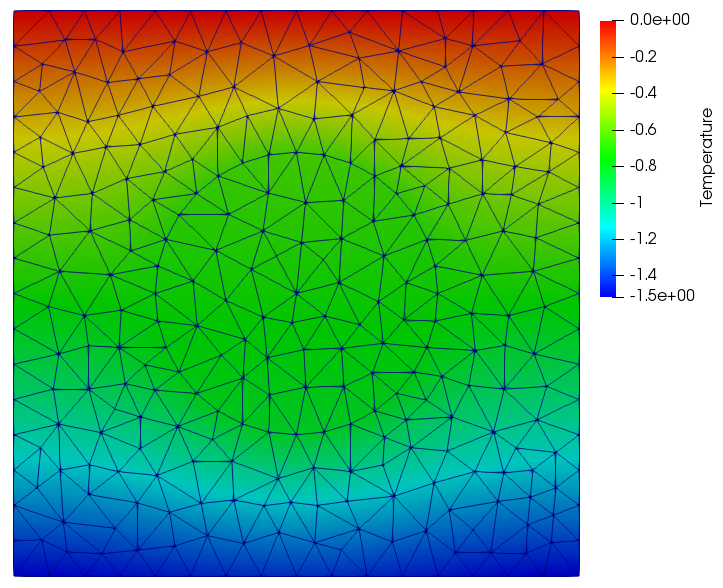
\includegraphics[width=0.5\textwidth]{figures/Thermal_Block.png}
        \caption{Representative solutions for the parametrized conductivity problem for $\mathbf{\mu} = (8.0,-1.0)$.}
        \label{fig:2}
    \end{figure}

To \textit{a posteriori} compare the error between the RB model and high-fidelity model, the maximum and average absolute errors with respect to number of selected basis functions were analysed. These metrics are defined as follows
\begin{align}
  Error_{max} = \max_{\mu \in \mathbb{P}_h} \|u_{\delta}(\mu) - u_{rb}(\mu)\| \\
  Error_{ave} = \frac{1}{|\mathbb{P}_h|} \sum_{\mu \in \mathbb{P}_h} \|u_{\delta}(\mu) - u_{rb}(\mu)\|
\end{align}
where $\mathbb{P}_h$ denotes the size of the testing set which in this case was selected to be 100 combinations of uniform random samples of parameter $\mathbf{\mu}$. The results are shown in fig.~\ref{fig:tb_err}
    \begin{figure}[h!]
        \centering
        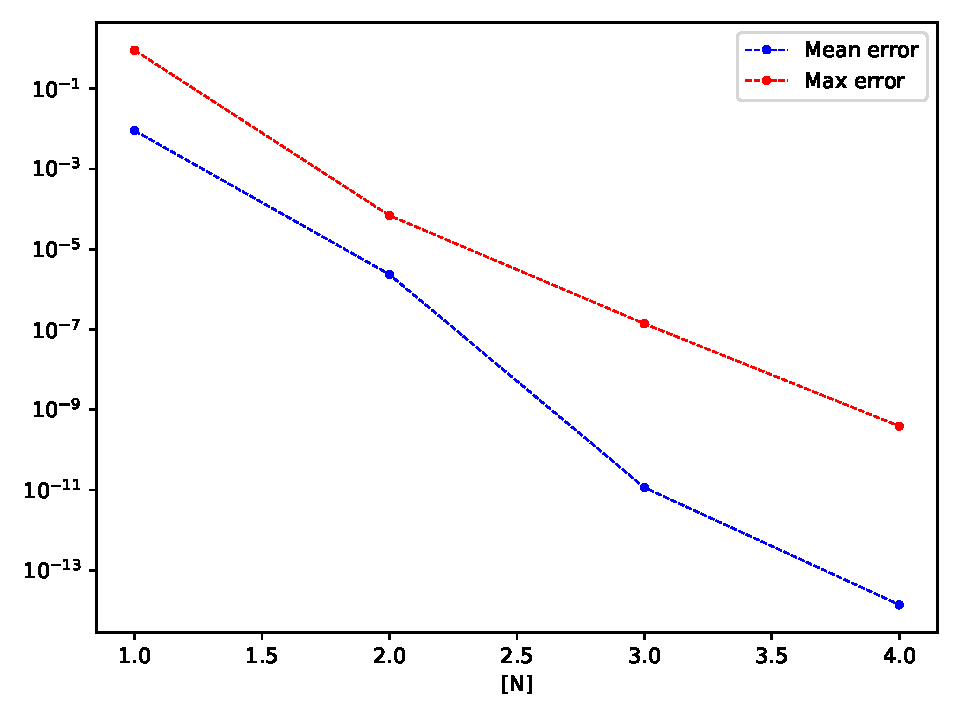
\includegraphics[width=0.75\textwidth]{figures/output_error.pdf}
        \caption{Maximum and average absolute errors with respect to number of selected basis functions for heat conduction problem.}
        \label{fig:tb_err}
    \end{figure}

For the same testing set, the maximum, minimum and average speedups with respect to number of selected basis functions were analysed.  These metrics are defined as follows
\begin{align}
  Speedup_{max} = \max_{\mu \in \mathbb{P}_h} \frac{T_{RB}}{T_{HF}} \\
  Speedup_{max} = \min_{\mu \in \mathbb{P}_h} \frac{T_{RB}}{T_{HF}} \\
  Speedup_{ave} = \frac{1}{|\mathbb{P}_h|} \sum_{\mu \in \mathbb{P}_h} \frac{T_{RB}}{T_{HF}}
\end{align}
where $T_{RB}$ and $T_{HF}$ denote the computation time required by the RB model and high-fidelity model respectively. The results are shown in fig.~\ref{fig:tb_spdup}
    \begin{figure}[h!]
        \centering
        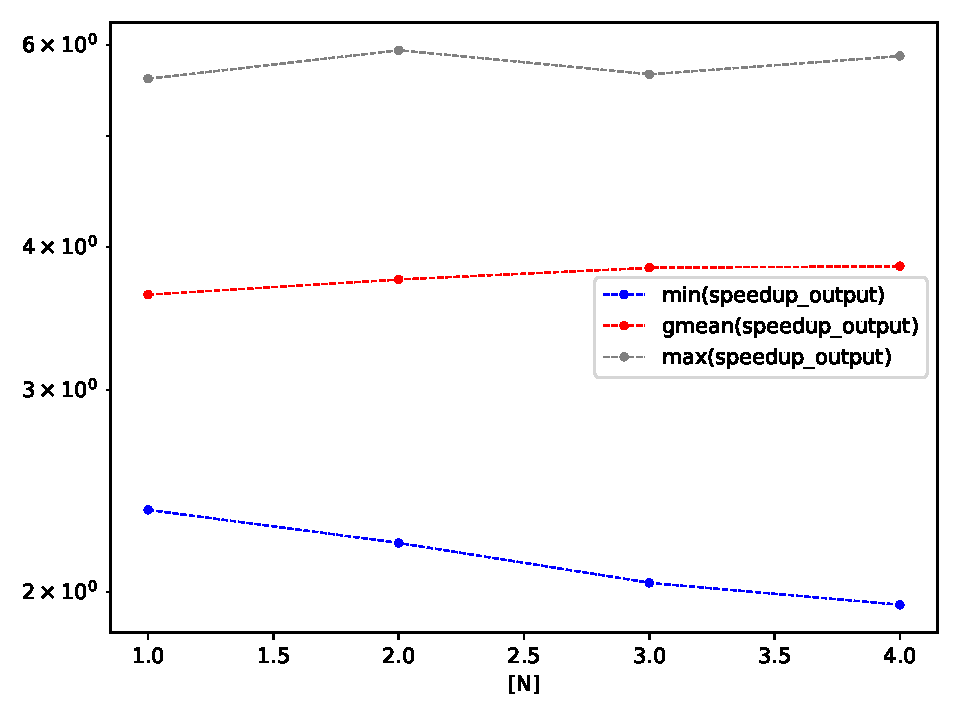
\includegraphics[width=0.75\textwidth]{figures/speedup_output.pdf}
        \caption{Maximum, minimum and average speedups with respect to number of selected basis functions for heat conduction problem.}
        \label{fig:tb_spdup}
    \end{figure}
The results show that for the heat conduction problem, the RB method performs as expected providing an average speedup of around $4\times$. The error while high for 1 and 2 basis functions, decays rapidly as the number of basis functions is increased. Thus, the RB method can be applied to speedup the heat conduction problem while maintaining sufficient accuracy.

\section{Fluid Flow in Backward Facing Step Channel}
A more complex problem where RB methods can be significantly useful is the fluid flow problem. For this demonstartion, the Navier-Stokes equations over the two-dimensional backward-facing step domain $\Omega$ shown in fig.~\ref{fig:NS}. A Poiseuille flow profile is imposed on the inlet boundary, and a no-flow (zero velocity) condition is imposed on the walls. A homogeneous Neumann condition of the Cauchy stress tensor is applied at the outflow boundary. The inflow velocity boundary condition is characterized by the following
\begin{equation}
  \boldsymbol{u}(\boldsymbol{x};\mu)=\mu\bigg \{\frac{1}{2.25}(x_1-2)(5-x_1),0\bigg \} \quad \forall \boldsymbol{x}=(x_0,x_1) \in \Omega
\end{equation}
and the problem is characterized by one parameter $\mu$, which characterizes the inlet velocity and $\mu \in [1.0, 80.0]$. Thus, the parameter domain is $\mathbb{P}=[1.0,80.0]$.
\begin{figure}
    \centering
    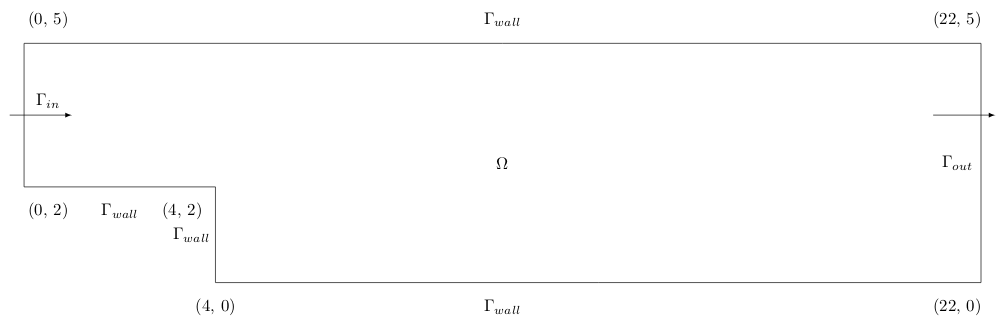
\includegraphics[width=0.75\textwidth]{figures/channel.png}
    \caption{Geometrical set-up of the fluid flow problem.}
    \label{fig:NS}
\end{figure}

\subsection{Parametrised formulation}
Let $\boldsymbol{u}(\mu)$ be the velocity vector and $p(\mu)$ be the pressure in the domain $\Omega$. The weak formulation for this problem is the following

For a given parameter $\mu \in \mathbb{P}$, find $u(\mu) \in \mathbb{V}(\mu), \; p \in\mathbb{M}$ such that
\begin{equation}
  \begin{cases}
    \nu \int_{\Omega} \nabla \mathbf{u} \cdot \mathbf{v} \ d\Omega + \nu \int_{\Omega}[(\mathbf{u}\cdot\nabla)\mathbf{u}]\cdot\mathbf{v} \ d\Omega - \int_{\Omega} p \nabla \cdot \mathbf{v} \ d\Omega = \int_{\Omega} \mathbf{f} \cdot \mathbf{v} \ d\Omega, /; \forall v \in \mathbb{V} \\
    \int_{\Omega} q \nabla \cdot \mathbf{u} \ d\Omega, /; \forall q \in \mathbb{M}
  \end{cases}
\end{equation}

where, $\nu$ represents kinematic viscosity, the functional space $\mathbb{V}(\mu)$ is defined as $\mathbb{V}=[H^1_{\Gamma_{wall}}(\Omega)]^2$ and the functional space $\mathbb{M}(\mu)$ is defined as $\mathbb{M}=L^2(\Omega)$.

\section{Implementation and results}
The implementation of the RB method using POD to generate upto 10 basis functions was performed using RBniCS. Since the affine decomposition is not explicit like the previous case and was computed by RBniCS. The solution for $\mu = 80.0$ has been shown in fig.~\ref{fig:NS_up}. The model was tested using the error and speedup estimates described in the previous section and are shown in figs.~\ref{NS:err_u}--\ref{fig:NS_spdup}.
\begin{figure}
    \centering
    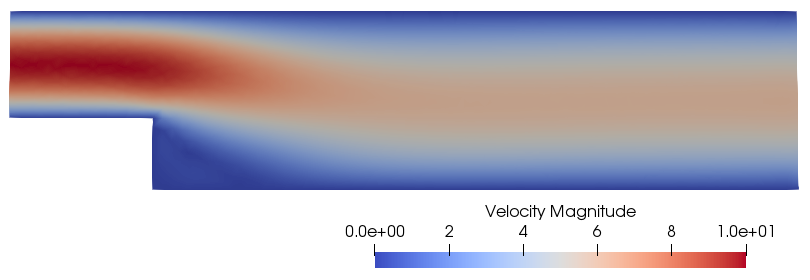
\includegraphics[width=0.85\textwidth]{figures/NS_velocity.png}\\
    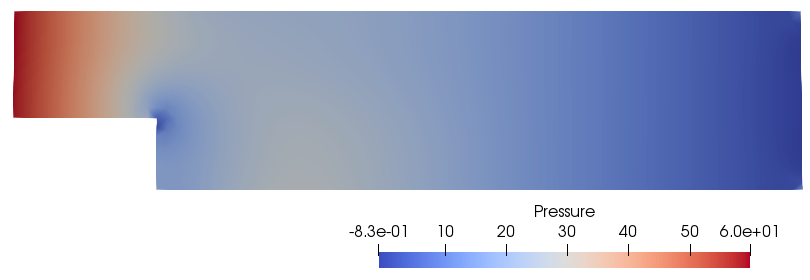
\includegraphics[width=0.85\textwidth]{figures/NS_pressure.png}
    \caption{Velocity magnitude and pressure distribution for the fluid flow problem for ${\mu} = 80.0$.}
    \label{fig:NS_up}
\end{figure}

\begin{figure}[h!]
    \centering
    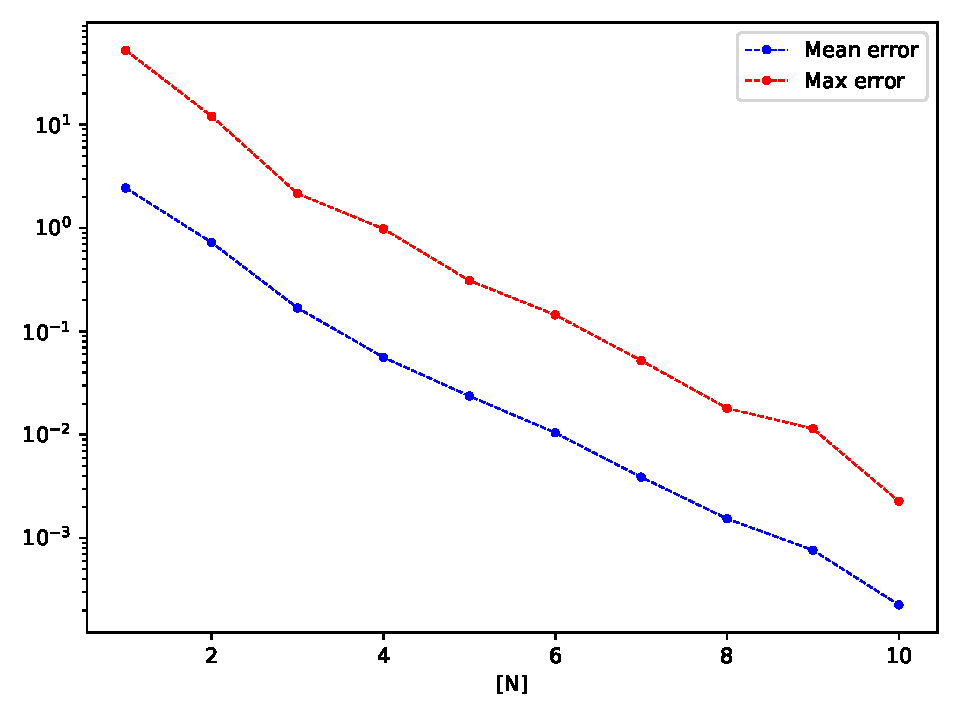
\includegraphics[width=0.75\textwidth]{figures/output_error_u.pdf}
    \caption{Maximum and average absolute errors in velocity with respect to number of selected basis functions for fluid flow problem.}
    \label{fig:NS_err_u}
\end{figure}

\begin{figure}[h!]
    \centering
    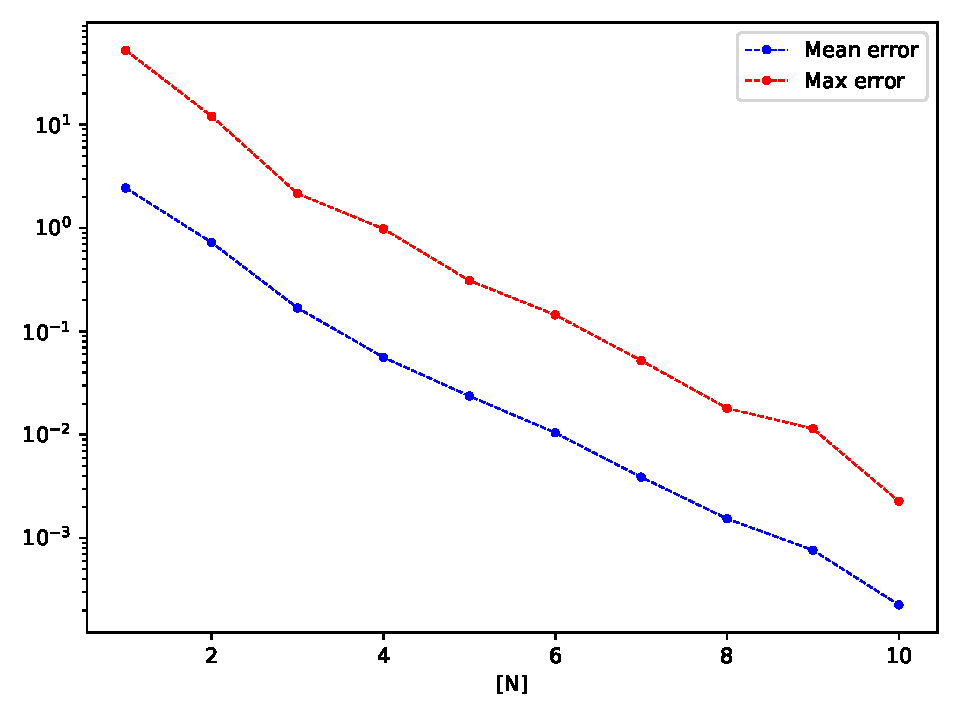
\includegraphics[width=0.75\textwidth]{figures/output_error_p.pdf}
    \caption{Maximum and average absolute errors in pressure with respect to number of selected basis functions for fluid flow problem.}
    \label{fig:NS_err_p}
\end{figure}

\begin{figure}[h!]
    \centering
    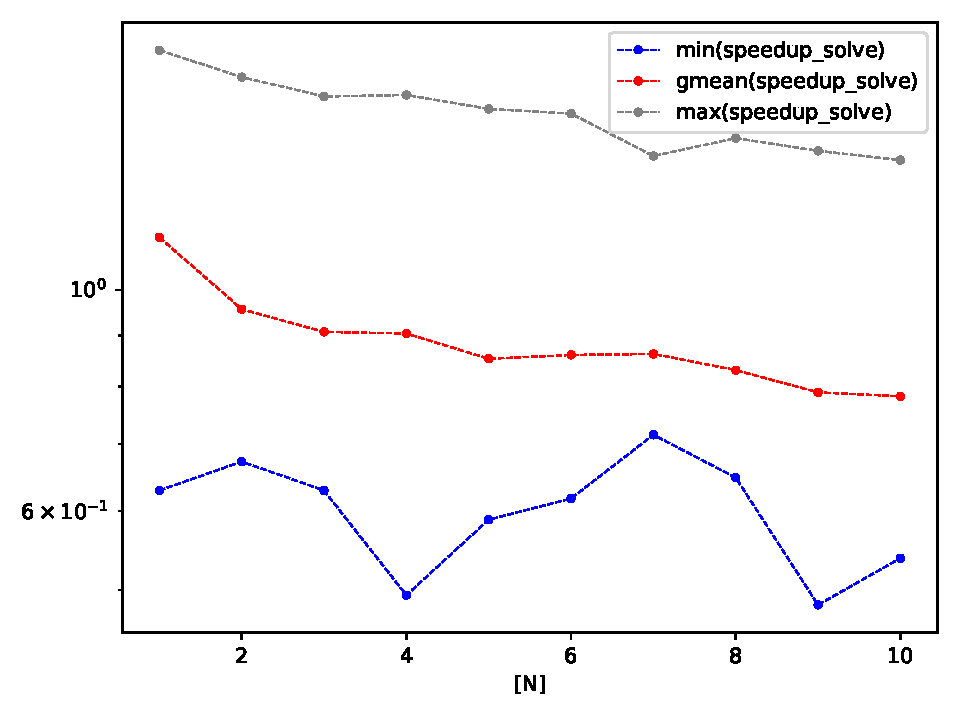
\includegraphics[width=0.75\textwidth]{figures/speedup_solve.pdf}
    \caption{Maximum, minimum and average speedups with respect to number of selected basis functions for fluid flow problem.}
    \label{fig:NS_spdup}
\end{figure}

While the errors are of the order of $10^{-3}$, using the RB method for the problem led to slowdown instead of speedup. This can be attributed to use of relatively small number of basis functions, use of the simplest affine decomposition and RB computation methods and also the non-linearity of the problem.

\section{Conclusion}
This project demonstrated the use of RB method in reducing the computational cost associated with multi-query computations of high-fidelity parametrised models. While the method was successfully demonstrated for a heat conduction toy problem, the fluid flow problem gave less than inspiring results. However, since a number of more sophisticated models are available in literature, this must not be seen as a failure of the RB approach. In fact, as shown by the heat conduction problem, these methods can be quite useful for many problems which explains the persistent interest in RB methods amongst the mathematics and engineering researchers.

  \bibliographystyle{ieeetr}
  \bibliography{references}
\end{document}
